%% This is file `medima-template.tex',
%%
%% Copyright 2018 Elsevier Ltd
%%
%% This file is part of the 'Elsarticle Bundle'.
%% ---------------------------------------------
%%
%% It may be distributed under the conditions of the LaTeX Project Public
%% License, either version 1.2 of this license or (at your option) any
%% later version.  The latest version of this license is in
%%    http://www.latex-project.org/lppl.txt
%% and version 1.2 or later is part of all distributions of LaTeX
%% version 1999/12/01 or later.
%%
%% The list of all files belonging to the 'Elsarticle Bundle' is
%% given in the file `manifest.txt'.
%%
%% Template article for Elsevier's document class `elsarticle'
%% with harvard style bibliographic references
%%
%% $Id: medima-template.tex 153 2018-12-01 11:38:32Z rishi $
%% $URL: http://lenova.river-valley.com/svn/elsarticle/trunk/medima-template.tex $
%%
%% Use the option review to obtain double line spacing
%\documentclass[times,review,preprint,authoryear]{elsarticle}

%% Use the options 'twocolumn,final' to obtain the final layout
%% Use longtitle option to break abstract to multiple pages if overfull.
%% For Review pdf (With double line spacing)
%\documentclass[times,twocolumn,review]{elsarticle}
%% For abstracts longer than one page.
%\documentclass[times,twocolumn,review,longtitle]{elsarticle}
%% For Review pdf without preprint line
%\documentclass[times,twocolumn,review,nopreprintline]{elsarticle}
%% Final pdf
\documentclass[times,twocolumn,final]{elsarticle}
%%
%\documentclass[times,twocolumn,draft,longtitle]{elsarticle}
%%


%% Stylefile to load MEDIMA template
\usepackage{medima}
\usepackage{framed,multirow}
\graphicspath{{./}{../../templates/MEDIMA-template/}{figures/}}
\usepackage{amssymb,latexsym}
\usepackage[nointegrals]{wasysym}

% Following three lines are needed for this document.
% If you are not loading colors or url, then these are
% not required.
\usepackage{url}
\usepackage{xcolor}
\usepackage{graphicx,amsmath}
\usepackage{subcaption}

\usepackage{hyperref}
\usepackage[nameinlink]{cleveref}
\Crefname{lstlisting}{listing}{listings}
\Crefname{lstlisting}{Listing}{Listings}

\usepackage{tikz}
\usetikzlibrary{positioning,arrows,calc}
\usepackage{listings}
%\renewcommand{\ttdefault}{pcr}
\lstset{
  numbers=left,
  captionpos=b,
  keepspaces=true,
  basicstyle=\scriptsize\ttfamily,
  keywordstyle=\bfseries\ttfamily,
  commentstyle=\color{gray}\ttfamily
}
\usepackage{algorithm}
\usepackage[noend]{algpseudocode}

\definecolor{newcolor}{rgb}{.8,.349,.1}

\journal{Medical Image Analysis}


\usepackage{tikz}
\usetikzlibrary{shapes.geometric}
\usetikzlibrary{arrows.meta,arrows}
\usetikzlibrary{positioning}


% \usepackage{showframe} % for debugging
\usepackage{ulem}
\newcommand{\carl}[1]{\textcolor{orange}{[Carl: #1]}}
\newcommand{\aleksandar}[1]{\textcolor{cyan}{[Aleksandar: #1]}}
\newcommand{\james}[1]{\textcolor{red}{[James: #1]}}
\definecolor{ForestGreen}{RGB}{34,139,34}
\newcommand{\suggestion}[3]{\textcolor{ForestGreen}{[\textbf{Suggestion (#1):} '\sout{#2}' $\rightarrow$ '#3']}}


\newcommand{\xx}{\mathbf{x}}
% \newcommand{\fval}{f(\xx)}
% \newcommand{\fval}{f}
\newcommand{\fval}{x}
\newcommand{\lab}{\mathrm{L}}
\begin{document}

\verso{Given-name Surname \textit{et~al.}}

\begin{frontmatter}

% \title{Spatial Analysis for SR$\mu$CT Segmentation}%
\title{
  Reversing distortive X-ray effects I:
  Accurate Implant-contact Tissue Classification in Bone SR$\mu$CT
}%

\author[1,2]{James \snm{Avery}\corref{cor1}}
\cortext[cor1]{Corresponding author:\\
  Address: Universitetsparken 5, 2100 Copenhagen O, Denmark \\
  Email: avery@nbi.ku.dk\\
}
\ead{avery@nbi.ku.dk}
\author[2]{Aleksandar \snm{Topic}}
\ead{aleksandartpc@gmail.com}
\author[1]{Carl-Johannes \snm{Johnsen}}
\ead{carl-johannes@di.ku.dk}
\author[3]{Else \snm{Pinholt}}
\ead{empinholt@health.sdu.dk}

\address[1]{University of Copenhagen, Department of Computer Science}
\address[2]{University of Copenhagen, Niels Bohr Institute}
\address[3]{University of Southern Denmark}

\received{30 June 2022}
%\finalform{10 May 2013}
%\accepted{13 May 2013}
%\availableonline{15 May 2013}
%\communicated{S. Sarkar}


\begin{abstract}
  %%%
  Synchrotron Radiation micro-CT (SR$\mu$CT) produces images at
extremely high fidelity.  However, while distortive X-ray effects such
as beam-hardening are minimized due to highly brilliant monocromatic
beams, they are not eliminated. In particular, obtaining accurate
tissue classification is a challenge near high-contrast interfaces
such as metal implants.

We present a computational method that discovers the image distortion as a function of space,
and produces continuous probabilistic models of material classification functions.
Using the derived models, we are able to accurately classify tissue throughout the full
image, even at high-contrast transition interfaces.
% 
We apply the method to solve the notoriously difficult problem of accurately classifying
biological tissue in contact with a titanium implant. 
  
{\bf The data:}
The new tissue classification method was aplied to evaluate
bone-to-implant contact (BIC) in micrometer-resolutiom SR$\mu$CT images.
In a previous study\cite{sporring}, we were unable to obtain accurate
results for BIC, due to difficulties in accurately classifying the
tissue types near the titanium implant surface. In the present work,
we fully reverse the distortive effects and obtain accurate tissue classification
all the way to the implant surface.

The method is implenented in C++ and Python, and is parallelized for GPU and multicore CPU.
To deal with the very large image sizes arising from SR$\mu$CT, exceeding system
memory on even large workstations, the algorithms are designed to run
out-of-core on multi-resolution representations of the tomograms.

The source code is available as open source at http://github.com/jamesavery/SASS/.



%%% Local Variables:
%%% mode: latex
%%% TeX-master: "main"
%%% End:

%%%%
\end{abstract}

\begin{keyword}
%% MSC codes here, in the form: \MSC code \sep code
%% or \MSC[2008] code \sep code (2000 is the default)
%\MSC 41A05\sep 41A10\sep 65D05\sep 65D17
\MSC 92C55\sep 62H35\sep
%% Keywords
\KWD Image analysis \sep Tissue classification \sep Ossointegration \sep Segmentation \sep Bone-to-implant contact \sep Synchrotron Radiation micro-CT
\end{keyword}

\end{frontmatter}

%\linenumbers

\section{Introduction}
\label{sec:intro}


\subsection{Image data}

Bone samples are most commonly analysed by extracting histologies and examining their
two-dimensional structure with light microscopy. This method has several drawbacks. First and
foremost, it is destructive: In addition to the obvious issue that the histology must be cut
from the full sample, the sawing process can contaminate soft tissue with bone dust, or leave
surface scratches that complicate automatic image analysis. Secondly, histology by its nature
only gives a two-dimensional slice of the full three-dimensional picture. Most important
biological structures are inherently three-dimensional, and limiting analysis to 2D severely
restricts the types of questions we can answer.

Synchrotron Radiation micro-tomography (SR$\mu$CT) offers a non-destructive high-quality
alternative to histology for detailed analysis of bone biopsies. \cite{torsten2018}
quantified the uncertainty of 2D histology for four common bone analyses, and found that the
choice of sampling plane for histological analysis incurred a significant uncertainty in the
results, whereas the full volumetric analysis of SR$\mu$CT tomograms did not.

The high brilliance and collimation of synchrotron radiation yields particularly
faithful 3D images, as common distortive X-ray effects seen in hospital-grade setups such
as beam hardening and projection artefacts are minimized. The high fidelity makes SR$\mu$CT
attractive for conducting advanced medical image analyses with trustworthy results.

However, while image distortion effects are much reduced compared to laboratory X-ray tomography,
they are not eliminated, and numerical analysis and computations on the images must still be
conducted carefully. Boundary effects near sample surfaces, ring artefacts from sensor faults, and especially
distortion near high-contrast transitions, make accurate tissue classification difficult in
regions where this distortion is significant. \cite{sporring} found that, while
they could accurately classify bone tissue in the middle regions of the tomograms, they were
not able to obtain good bone-to-implant contact evaluation (BIC), as evidenced by poor correlation
with histological analysis of the same samples.

The present work presents a fully automatic computational method which discovers probabilistic
models for the distortions incurred by the physical effects in high-resolution X-ray CT such
as SR$\mu$CT in order to reverse them and produce accurate tissue classification even in regions
where these effects are significant. It exploits two properties, which are needed to hold for
the method to work: i) very high resolution is used to build statistical models as functions
of space, and ii) the effects to be countered must vary continuously over space, so that we can
track how voxel frequency distributions are distorted throughout the image.
We apply the method to the
same dataset of micrometer-resolution SR$\mu$CT bone tomograms studied in \cite{torsten2018}
and in \cite{sporring}, to achieve faithful tissue classification all the way to the titanium
implant surface.

Our goal is to obtain good conditional probability distributions $P(m|v,\xx)$
that model the likelihood of a voxel having material type $m$ as a function
both on its value $v$ and its position $\xx$ in the tomogram. We want to make sure that these distribution
functions vary smoothly across space, to ensure that we can identify the materials correctly across the entire
image: even though the frequency distributions look completely different
close to the titanium implant compared to the middle region or sample surface,
we can track the unbroken, smooth deformation to assign a global material
identity.

The aims of the current work is:
\begin{enumerate}
\item To design a fully automatic \textbf{spatially aware segmentation algorithm} that
  improves segmentation quality of tissues in bone-SR$\mu$CT in all regions, including near high-contrast interfaces.
\item To implement this method efficiently in open-source software for GPU and multi-core CPU using out-of-core techniques, to
  facilitate analysis of 3D SR$\mu$CT images that exceed system memory.
\item To use the new method to evaluate bone-to-implant contact closer to implant surfaces than previously feasible. 
\end{enumerate}




%%% Local Variables:
%%% mode: latex
%%% TeX-master: "main"
%%% End:


\section{Background}
\label{sec:background}

In this section, we will briefly go through the physical composition of our samples, and how the
data is acquired. Then we will look at the noise sources typical for this type of data, and show
the effects that noise has on regions around the implant and biological tissue.

\subsection{Data set}


Seven goats got introduced 5 critical size defects, with bone being cut accordingly in the region.
 Four defects were used to asses bone regeneration methods, and one was a control sample.
 Peri-implant vertical bone augmentation was performed using autologous bone and two different
 calcium phosphate bone substitutes. The bone specimens were evaluated undecalcified. The
 specimen preparation was performed at the Department of Biomaterials at Gothenburg University,
 Sweden. The specimens were initially fixated in 4\% paraformaldehyde. Dehydration of the
 specimens was performed in increasing concentrations of ethanol to eliminate fat and water
 content. Furthermore, specimens were infiltrated with MMA and embedded in molds 12 mm in
 diameter and 20 mm in height \james{(Donath 1982, 1993, Erben 1997)}. They were scanned at the ESRF
 in Grenoble, France. The advantage of using MMA is greater tissue penetration than water-soluble
 methacrylates this is an advantage when preparing larger specimens such as bone biopsies
 containing dental implants. Furthermore, the histological quality of bone sections is generally
 higher for MMA embedded specimens compared to water- soluble methacrylates \james{(Erben 1997)}.
 Additionally, tissue shrinkage is less than 2\% when using MMA embedded bone and cartilage
 specimens \james{(Ferguson et al. 1999)}.


As the specimen for X-ray imaging included a titanium dental implant, comparatively high photon
 energy of 50 KeV (pink) was chosen, i.e. the
 emitted radiation of a wiggler insertion device (a
 magnetic device) was filtered    to produce a narrower bandwidth. An indirect detector (lens-coupling
 of a scintillator to a camera incorporating a charge-coupled device with $2048 \times 2048$ pixels),
 with a pixel size of 5$\mu$m acquired tomographic scans of the ROI, which was slightly smaller (10mm wide)
 than the specimen (~20mm wide)” (Neldam et al. 2015). The sample was continuously rotated over
 180 degrees, as 1999 equiangular spaced radiographic images were taken.

\subsubsection{Physical samples}

The physical samples were prepared for SR$\mu$CT scanning by cutting out a portion from a larger
12mm cylindrical sample. The cut samples are cubes of size (6.478mm, 6.478mm, 6.146mm) in the
$(x,y,z)$ direction respectively. This contains the titanium dental implant (Astra Tech OsseoSpeed,
ST Molndal, Sweden), which is 3.5mm in diameter and 8mm long. Along its length the lower 5.5mm
has larger threads and is attached to recipient bone. The upper 2.5mm has smaller threads and
is where newly formed bone is to be assessed. Sorrounding the bone and implant contact-region
are cavities containing resin, air, blood vessels and other fibrous tissue.

\begin{figure}
\centering
\includegraphics[width=0.96\columnwidth]{770c_pag-full-xy-1x.png}
\includegraphics[width=0.96\columnwidth]{770c_pag-full-yz-1x.png}
\includegraphics[width=0.96\columnwidth]{770c_pag-full-xz-1x.png}
\caption{Cut sample seen as cross sections in XY, YZ and XZ-planes respectively. A voxel has a size
of 1.875$\mu$m. Red voxels are numerically low, while blue voxels are high.}
\label{fig:3viewsample}
\end{figure}

A cut sample is shown in three different cross sectional views in \Cref{fig:3viewsample}. Each
material has a unique density and thus absorption. The titanium implant shown in blue has a
higher absorption level than bone. Bone material shown in light orange has higher absorption
than its sorrounding dark orange colored regions containing blood vessels tissue, air and resin.

\subsubsection{Data acquisition}

It can be difficult to study and evaluate the bone structure and blood network without destroying
or manipulating the sample. X-ray computed tomography is a widely used tool for non-intrusive medical
imaging. By exposing a subject to X-rays, we can map the linear attentuation coffecient of the passing
rays. Each ray is attenuated relatively to the density and composition of the material it passes.
By rotating either the scanner or the sample we can get a full 3D image representation of the inner
structure of the sample. Each volumetric pixel (voxel) then represents the X-ray attenuation at its
spatial position. We can therefore reliably use X-rays to internally characterise samples in a
non-intrusive and non-destructive manner. Medical CT-scans can provide spatial resolutions on the
order of submillimetre scale \citep{medicalct}. The more modern micro computed tomography ($\mu$CT)
can provide much higher spatial resolution on the micrometre scale \citep{srexptime}.

This work focuses on a data set acquired by Synchrotron Radiation micro-CT (SR$\mu$CT). For this
imaging technique, electrons are accelerated to ultra-relativistic speeds in trajectories directed
by strong magnetic fields. The resulting X-ray beam provides a high photon flux allowing for very
short exposure times \citep{srexptime}. This can help counter Poisson noise from suboptimal photon
count \citep{srnoise}. Contrary to both CT and $\mu$CT, this approach requires a large particle
accelerator, and is not standard medical or laboratory equipment. However, SR$\mu$CT  offers an
even better spatial resolution of up to 0.1 $\mu$m, and much higher image quality due to fewer
distortive X-ray effects. The resulting beams are high in brilliance and collimation, which gives
a very clear signal. Artifacts from beam-hardening are minimized due to synchrotron radiation
X-rays being characeterised by their practially mono-energetic spectrum.

The tomograms prestened here have been acquired at the ID19 beam line at the European Synchrotron
Radiation Facility (ESRF) in Grenoble, France. They were reconstructed\citep{sporring} at the
ID19 beamline. A standard filtered back-projection algorithm was applied via the ESRF in-house developed
software PyHST\citep{pyhst}. PyHST was applied to improve reconstruction quality, hence reducing ring
artefacts, and to reduce the required data volume if necessary \james{(Mirone et al. 2014)}. The
size of the reconstructed tomogram was $2048 \times 2048 \times 1024$ voxels. The segmentation was
performed using VG Studio Max 2.1 (Volume Graphics GHBM, Heidelberg, Germany) also at the ESRF in
Grenoble, France. The tomograms were acquired at 50 KeV.

\subsubsection{Image data}

The full physical size of a sample is about 6.5mm in each direction. Each image sample contains
voxels with a spatial resolution of 1.875$\mu$m. The samples are scanned in chunks of 4-6
sub-volumes through the height of the implant, depending on the initial size of a sample.
For computational purposes, the pixel size has been cropped to be divisible by a power $2^N$ or
more specifically $2^5=32$ was used in our case. This gives a size of $(3456,3456,846)$ pixels
per sub-volume, where the last axis gets stacked for a full volume. This makes the raw dimensions
of a single image containing 4 subvolumes $(3480,3480,3384)$ pixels in total. Before being stacked,
we need to volume match any overlapping regions. The overlaps are only shifted in the last dimension.
This made it possible to find the best overlap by simply minimizing the pixel-wise Eucledian distance
between the volumes. The size of the shifted volumes goes from $846 \rightarrow 810$.

In image \Cref{fig:3viewsample} (YZ and XZ planes) we can clearly see darker edges around the border
of the volume matched subvolumes at their overlaps. This creates an offset which is strongly seen
within the implant, but the large contrast due to very high density, makes this easier to ignore.
Even worse is the contribution of misrepresented voxels in the transitional regions where bone and
tissue contains these jagged edges.

\subsection{Physical effects, noise and artifacts}
\label{sec:physics}

Noise in tomography is unavoidable, and it makes segmentation harder because it further obscures
the boundaries between materials. Matarials may be well separated from certain angles in the
3d-reconstructed image, but overlap from others. Some noise like that corrected by flat-field
correction is very uniformly distributed across images. Some noise is however very spatially
dependent on its sorrounding regions. Knowing the composition and positioning of the materials
being imaged, we can counter some of these effects during segmentation. The noise effects manifest
themselves as numerical shifts in voxel-values as a function of their position. This is a direct
result of a misrepresented attenuation along the axis the X-rays are passing.

This orientation dependency illustrates how voxel intensity values are not globally fixed. How a
certain material is represented in intensity, is highly dependent on its position relative to
neighbouring regions. Especially since this also determines the amount and type of derived noise.
The same material with the same density, can thus be represented at multiple varying intensities
within the same sample.

\begin{figure*}
\centering
\includegraphics[width=\textwidth]{770c_pag-bic-xy-1x.png}
\caption{Here we see a 1mm x 2mm region of an unscaled image slice in the XY dimension. It highlights
some of the imperfections and noise present in the data. We especially see artifacts within and
around the titanium implant.}
\label{fig:xy-slice}
\end{figure*}

In \Cref{fig:xy-slice} and \Cref{fig:yz-slice} we see zoomed in regions of the XY and YZ planes
of the same sample as shown in \Cref{fig:3viewsample}.
Both planes display a broad selection of the various type of noise sources found in the data.

\begin{figure}
\centering
\includegraphics[width=\columnwidth]{770c_pag-bic-yz-1x.png}
\caption{Here we see a 1.5mm x 1.5mm region of an unscaled image slice in the YZ dimension. This
hightlights noise and voxexl effects around the newly formed bone in the micro threaded part of
the titanium implant.}
\label{fig:yz-slice}
\end{figure}


\subsubsection{Ring artifacts}

Looking at the XY-slice in \Cref{fig:xy-slice} we see clear concentric ring artifacts emanating from
the center of the sample, and at strong edges of the titanium implant. It propagates strongly through
the large region of air behind the implant. Compared to the other artifacts mentioned, this effect is
arising from imperfections in the scanner setup. These types of artifacts can typically come from
uncalibrated or defect adjacent detector elements. For synchrotron radiation sources it can also
occur from shifts and vibrations in the monochromator crystal \citep{ringartifacts}.

\subsubsection{Projection artifacts}

Bright streaks with strong edges are seen from the sharp corners of the titanium implant. When
doing back projection, the symmetry breaking is seen as smeared lines across the sample. This
can occur from the high pass filter used during filtered back projection, which exaggerates the
differences between adjacent elements \citep{ctnoise}.

\subsubsection{Compton scattering}

Lower energy rays contribute mostly with noise from scattering effects. A ray will propagate through
a material, get scattered and diffract from its initial trajectory. This gives a misrepresentation
of the attenuation along its initial trajectory. The artefacts seen from scattering are similar in
nature to those formed by beam hardening. This is because both effectively reduce the measured
attenuation. For energy levels of above 50KeV relevant for the data presented here, Compton
scattering is the dominating type \citep{compton}. The scattering occurs due to photon-electron
interaction between X-ray beam and the material it passes through. Like beam-hardening, scattering
will cause dark streaks across the image, where attenuation was highest.

\subsection{Beam hardening}\label{sec:beam-hardening}

Medical CT and $\mu$CT both utilize poly-energetic beams, which can cause artifacts around high
density regions. This effect is called beam-hardening \citep{beamhardening}, and occurs when rays
with lower energy are attenuated more frequently, thus shifting the remaining photon energy to a
higher effective average value. This offsets the local contrast, by overestimating the attenuation,
leaving lighter spots on the image. Many types of artifacts will typically be present in these
setups, but most are taken into account by calibration using phantoms and pre-hardening the beam
before it reaches the sample. Pre-hardening of the beam is done using filters that attenuate the
softest rays. Due to its common usage, various metal artifact reduction (MAR) software exists to
account for noise and imperfections during reconstruction \citep{mar1}\citep{mar2}.

Despite the practially mono-energetic rays from SR$\mu$CT, the source initially generates a
polychromatic spectrum. During monochromatisation the resulting spectrum can still contain
corrupted harmonic components. Only a few percent corruption is enough to produce strong
artifacts, although monochromatisation is typically done in multiple layers \citep{srnoise}.
It can not trivially be rejected that some noise does occur from poly-energetic incident radiation.
Two distinct effects typically seen as a result of beam-hardening are in dark and bright streaks
and cupping artifacts in high density regions.

\subsubsection{Dark and bright streaks}

Streaking artifacts occur at the dense implant region, but also in the transition from bone to softer
tissue. This effect is mostly seen in regions of large heterogeneity. When X-ray beams pass at angles
containing multiple dense obstacles, the beam is hardened more. Then for angles with fewer dense
obstacles the energy spectrum is preserved better. This produced the dark and bright streaks seen in
\Cref{fig:xy-slice}.

For a hardened beam, softer x-rays are absorbed instead of successfully penetrating the object,
and will not contribute to image formation. High density structures such as the titanium implant
break the isotropy, making the projected X-ray mean energy spectrum dependent on incident orientation
\citep{srnoise}.

\subsubsection{Cupping effect}

A common artefact that occurs when beams pass more homogeneous cylindrical objects. Since beams
passing the middle will traverse more material compared to the edges, the beam is hardened more
towards the center and intensity becomes lower as a result. This can manifest itself in what
errnoeously looks to be dense peripheral regions at the edges.

\subsection{Phase contrast}

Phase contrast is an effect whose consequences are not very unlike those of beam-hardening.
Although used as an advantage in holotomography\citep{holotomography} and phase contrast tomography\citep{phasecontrast},
it induces noise in regular tomography such as used here. It typically results in fringes around edges
of regions within the image\citep{srnoise}. Similar to dark and bright streaks mentioned above,
they show as misrepresentations of the voxel values. In our case we see them especially at the
transitional edges between the titanium implant and the biological tissue and bone.

%Partial volume artifacts which are dependent on the voxel size and are mentioned briefly by Neldam et al.

%%% Local Variables:
%%% mode: latex
%%% TeX-master: "main"
%%% End:


\section{Physical effects}
\label{sec:physics}

Noise in tomography is unavoidable, and it makes segmentation harder because it
further obscures the boundaries between materials. Materials may be well
separated from certain angles in the 3D-reconstructed image but can overlap
from other angles. Some noise is very uniformly distributed across images, such
as the noise removed by flat-field correction, while other noise is very
spatially dependent on its surrounding regions. Knowing the composition and
positioning of the materials being imaged, we can counter some of these effects
during segmentation. The effects from noise manifest themselves as numerical
shifts in voxel values as a function of their position. This is a direct result
of a misrepresented attenuation along the axis the X-rays are passing.

This dependency on orientation illustrates how voxel intensity values are not
globally fixed. Instead, how a certain material is represented in intensity, is
highly dependent on its position relative to neighboring regions. Especially
since this also determines the amount and type of derived noise. The same
material with the same density can thus be represented at multiple varying
intensities within the same sample.

\begin{figure}
  \centering
  \begin{tabular}{cc}
    \!\!\!\!\!\!(a)\!\!\!&\begin{tabular}{c}\includegraphics[width=0.85\columnwidth]{generated/770c_pag_roi_yx.pdf}\end{tabular}\\
    \!\!\!\!\!\!(b)\!\!\!&\begin{tabular}{c}\includegraphics[width=0.85\columnwidth]{generated/770c_pag_roi_zy.pdf}\end{tabular}\\
  \end{tabular}
  \caption{
    To better see the distortion effects, we zoom in on two sub-regions of the
    slices shown in \Cref{fig:3viewsample}. Our visual systems automatically
    correct for most of the distortions, as they appear similar to illumination
    effects. However, even some distance from the implant, blood vessel voxels
    have higher values than bone voxels further out. As we approach the
    implant, the value shifts accelerate and become highly non-linear.
    % TODO highlight this using arrows and absolute values?
    (a) A 1 mm $\times$ 2 mm region of an image slice in the YX-plane.
    % It highlights some of the imperfections and noise present in the data.
    (b) A 1.5 mm $\times$ 1.5 mm region of an image slice in the ZY-plane in the
    micro-threaded part of the titanium implant.
  }
\label{fig:slices}
\end{figure}

In \Cref{fig:slices}, we see zoomed-in regions of the YX- and ZY-planes of the
same sample as shown in \Cref{fig:3viewsample}. Both planes display a broad
selection of the various types of noise sources found in the data.
\begin{itemize}
  \item \textbf{Beam hardening:} Medical CT and µCT both utilize poly-energetic
      beams, which can cause artifacts around high-density regions. This effect
        is called beam-hardening \citep{beam-hardening}, and occurs when rays
        with lower energy are attenuated more frequently, thus shifting the
        remaining photon energy to a higher effective average value. This
        offsets the local contrast, by overestimating the attenuation, leaving
        lighter spots on the image. Many types of artifacts will typically be
        present in X-ray setups, but most are taken into account by calibration
        using phantoms and pre-hardening the beam before it reaches the sample.
        Pre-hardening of the beam is done using filters that attenuate the
        softest rays. Due to its common usage, various metal artifact reduction
        (MAR) software exists to account for noise and imperfections during
        reconstruction \citep{mar1}\citep{mar2}.

    Despite the practically mono-energetic rays from SRµCT, the source
        initially generates a poly-chromatic spectrum. During
        monochromatisation the resulting spectrum can still contain corrupted
        harmonic components. Only a few percent corruption is enough to produce
        strong artifacts, although monochromatisation is typically done in
        multiple layers \citep{srnoise}. It can not trivially be rejected that
        some noise does occur from poly-energetic incident radiation. Two
        distinct effects typically seen as a result of beam-hardening are the
        dark and bright streaks and cupping artifacts in high-density regions.

  \item \textbf{Dark and bright streaks:} Streaking artifacts occur at the dense
    implant region, but also in the transition from bone to softer tissue. This
        effect is mostly seen in regions of large heterogeneity. When X-ray
        beams pass at angles containing multiple dense obstacles, the beam is
        hardened more. Then for angles with fewer dense obstacles, the energy
        spectrum is preserved better. This produced the dark and bright streaks
        seen in \Cref{fig:slices}.
        %
        For a hardened beam, softer X-rays are absorbed instead of successfully
        penetrating the object, and will not contribute to image formation.
        High-density structures such as the titanium implant break the
        isotropy, making the projected X-ray mean energy spectrum dependent on
        incident orientation \citep{srnoise}.

  \item \textbf{Cupping effect:} A commonly occurring artifact is when beams pass
    more homogeneous cylindrical objects. Since beams passing the middle will
        traverse more material compared to the edges, the beam is hardened more
        towards the center and intensity becomes lower as a result. This can
        manifest itself in what erroneously looks to be dense peripheral
        regions at the edges.

  \item \textbf{Phase contrast:} Phase contrast is an effect whose consequences
    are not very unlike those of beam-hardening.  Although used as an advantage
        in holotomography\citep{holotomography} and phase contrast
        tomography\citep{phasecontrast}, it induces noise in regular tomography
        such as those used here. It typically results in fringes around the
        edges of regions within the image\citep{srnoise}. Similar to the dark
        and bright streaks mentioned above, they show up as misrepresentations
        of the voxel values. In our case, they are especially prominent at the
        transitional edges between the titanium implant and the biological
        tissue and bone.

  \item \textbf{Ring artifacts:} Looking at the XY-plane in
      \Cref{fig:slices}(a) we see clear concentric ring artifacts emanating
        from the center of the sample, and at strong edges of the titanium
        implant. It propagates strongly through the large region of air behind
        the implant. Compared to the other artifacts mentioned, this effect
        arises from imperfections in the scanner setup. These types of
        artifacts can typically come from uncalibrated or defect-adjacent
        detector elements. For synchrotron radiation sources it can also occur
        from shifts and vibrations in the monochromator crystal
        \citep{ringartefacts}.

  \item \textbf{Projection artifacts:} Bright streaks with strong edges are
      seen from the sharp corners of the titanium implant. When doing back
      projection, a symmetry break is seen as smeared lines across the sample.
      This can occur from the high pass filter used during filtered back
      projection, which exaggerates the differences between adjacent elements
      \citep{ctnoise}.

  \item \textbf{Compton scattering:} Lower energy rays mostly contribute noise
      from scattering effects. A ray will propagate through a material, get
      scattered and diffract from its initial trajectory. This gives a
      misrepresentation of the attenuation along its initial trajectory. The
      artifacts seen from scattering are similar in nature to those formed by
      beam hardening. This is because both phenomena effectively reduce the
      measured attenuation. For energy levels relevant to the data presented
      here, of 50 KeV and above, Compton scattering is the dominant type
      \citep{Compton}. The scattering occurs due to photon-electron interaction
      between the X-ray beam and the material it passes through. Like
      beam-hardening, scattering will cause dark streaks across the image,
      where the attenuation was highest.
\end{itemize}

The distortions that come from the class of physical effects and noise
artifacts discussed in this section, will vary continuously as a function of
the spatial coordinates. This allows the possibility for a method, which can
correctly identify materials despite varying voxel values.
% FIXME: Would like a reference for the continous argument
% It is also mentioned in the last sentences of the first paragraph in
% "Physical effects, noise and artifacts"

%Partial volume artefacts which are dependent on the voxel size and are mentioned briefly by Neldam et al.


%%% Local Variables:
%%% mode: latex
%%% TeX-master: "main"
%%% End:


\section{Method}\label{sec:method}
% Spatial correlation 2d histograms (den nemme, 1 2d hist)
In this section, we will describe the method for exploiting spatial correlation based of the 2D-histograms of the tomographies. 

\subsection{1-dimensional histograms}
%diskuter overlappende materialer
If we look at a 1D-histogram of a tomography, as shown in~\Cref{fig:1d-hist}, we see that it is hard to globally threshold which material belongs to which voxel intensity. 
This is because the voxel intensity is not a globally defined value, as explained in~\Cref{sec:physics}, which means that the different materials cover ranges of intensities, which blend together in the histogram.
Instead, we should exploit the spatial information in the tomography, as the intensities varies according based of off their positioning.  

\begin{figure}
    \centering
    \carl{TODO 1D histogram of a tomography. Skal måske have nogle fordelinger "fittet" ind, så man kan se overlappet?}
    \caption{1-dimensional histogram of a tomography. The x-axis depicts voxel intensity.}
    \label{fig:1d-hist}
\end{figure}

\subsection{Correlation of the different angles}
%Show the correlation of x,y,z,r to histograms 2d
In order to include spatial information, we consider \emph{expanding} a dimension to produce multiple 1-dimensional histograms.  
Each histogram is computed by locking the dimension in question and produce 
and combine these for each entry in the expanded axis into a new 2-dimensional histogram. 
We consider expanding four different axes of the tomography: x, y, z and radius (r). 
Each of them can be computed with a single pass over the entire tomography, as the code in~\Cref{lis:2dhists} shows. 
%discuss the effects with references to the physics (previous section)

\begin{figure}
    \begin{lstlisting}[language=Python,caption=Python-like pseudo code for computing 2D histograms.,label=lis:2dhists]
for z, y, x in indices:
    v = voxels[z,y,x]
    r = int(sqrt((x-cx)**2 + (y-cy)**2))
    zhist[z,v] += 1
    yhist[y,v] += 1
    xhist[x,v] += 1
    rhist[r,v] += 1
    \end{lstlisting}
\end{figure}

The four expanded histograms can be seen in~\Cref{fig:2dhists}. 
We can see that the different expansions divide the materials differently, based on where in the tomography we look.
E.g. the top part of the \texttt{y} histogram only has a single distinquishable material, whereas the bottom part carries multiple clearly distinquished materials. 

\begin{figure}
    \centering
    \carl{TODO four plots of the 2d histograms x, y, z, and r.}
    \caption{2D histograms of the different dimension expansions.}
    \label{fig:2dhists}
\end{figure}

\subsection{Removing unnecessary information.}
\carl{Mention how we apply the implant and bone masks? Or should it be before, so that the x,y,z,r histograms are also 2 materials?}

\subsection{EDT, diffusion}
%Show that the fields can perfectly seperate
%discuss all the way to implant contact
While the four histograms further seperate the materials at different angles, they are not good at depicting the materials close to the implant.


EDT is good overall, but difficult close to the implant. 

Use diffusion to "zoom in" on the implant, as it is good close to the implant, but throws everything far away into the same bin

Show that the distance to the implant in edt will be the same in the grooves of the screw compared to the threads of the screw. This is "fixed" with diffusion, as the grooves will be brigher as it is surrounded by more implant.

\subsection{Walkthrough of the method}

\subsubsection{Overview}
Coarse steps, explain the idea

steps -> flow chart
\begin{figure}
    \centering
    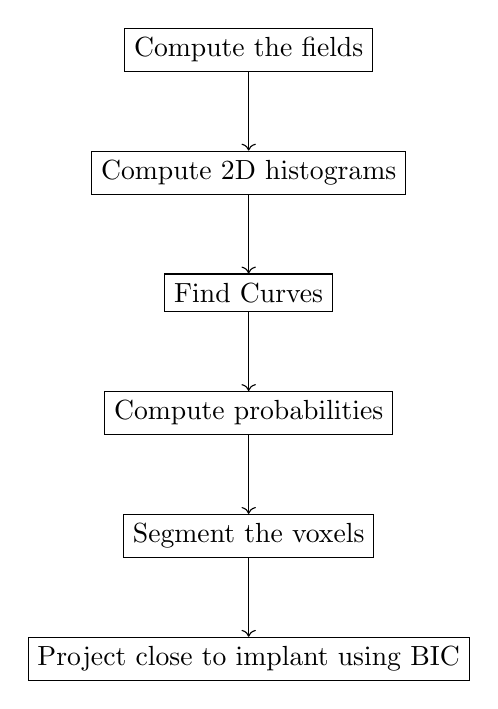
\begin{tikzpicture}
        \node[draw] (field) at (0,0) {Compute the fields};
        \node[draw, below = of field] (hists) {Compute 2D histograms};
        \node[draw, below = of hists] (curvs) {Find Curves};
        \node[draw, below = of curvs] (probs) {Compute probabilities};
        \node[draw, below = of probs] (segm) {Segment the voxels};
        \node[draw, below = of segm] (bic) {Project close to implant using BIC};

        \path[draw, ->] (field) -- (hists);
        \path[draw, ->] (hists) -- (curvs);
        \path[draw, ->] (curvs) -- (probs);
        \path[draw, ->] (probs) -- (segm);
        \path[draw, ->] (segm) -- (bic);
    \end{tikzpicture}
    \caption{Flowchart depicting the steps of the method. 
    \carl{Skal nok labeles, så man nemt kan se hvilken section der beskriver det. Plus, teksten i kasserne nok også kan være mere flavorful!}
    \carl{Kan måske arrangeres ligesom Davids ting oversigt? Giver måske kun mening hvis der var mere end bare segmentation -> bic}}
    \label{fig:flowchart}
\end{figure}

\subsubsection{Segmentation}

\begin{description}
    \item[Field-computations]

    EDT

    Diffusion

    EDT + Diffusion

    (remember to show images)

    \item[2D histograms]

    \item[Curves]

    \item[Probabilities]
\end{description}

\subsubsection{BIC computations}

\subsection{Results of the field segmentation}



\section{Conclusion and future work}
\label{sec:conclusion}

While SR$\mu$CT yields 3D reconstructions of extremely high fidelity compared to lab-grade X-ray setups,
several distortion effects remain that obstruct accurate tissue classification in important regions, in particular
near and at interfaces of high-contrast transitions such as where biological tissue meets metallic implants.
However, these effects are well behaved, in the sense that they vary smoothly over space, making it possible
to discover approximate mathematical models of the effects, and counter their resulting distortion.

We were able to build probabilistic models for the distortive effects
of soft tissue and bone voxel values as functions of distance to the
implant, and as functions of an approximate diffusion field. This made
it possible to see all the way up to the implant surface, and
automatically segment into tissue types throughout the sample and all
the way up to the implant surface, with high accuracy both at long and
short distances.

In this pilot work, we have only made a qualitative study. In upcoming
work, we plan a larger quantitative study that compares with histology
microscopy results, obtained from the same biopsies.  In addition, we
are extending the method with Bayesian combination of multiple
``angles'': different sources of distortion effects (e.g.~multiple
physical effects) can be better captured by different fields,
e.g.~beam hardening may be best captured by the distance transform to
the sample surface, while the diffusion field captures distortion near
metallic implants. Thus different fields separate tissue material
distributions in different regions, and in combination are expected to
yield a stronger analysis. It is hoped that this will make it possible
to separate multiple highly overlapping frequency distributions.


\section{Acknowledgements}

This project has received funding from the European Union’s Horizon 2020 research and innovation programme under grant agreement No. 779322 (``MAXIBONE'').
JA was partially supported by the VILLUM Foundation through VILLUM Experiment Project: 41017.
CJ was funded by the Innovation Fund Denmark (IFD) under File No. 8057-00012B, the IFD Grand Solutions project ``Adaptive X-ray InSpection''.

\section{Conflict of Interest}
On behalf of all authors, the corresponding author states that there is no conflict of interest. 


%%% Local Variables:
%%% mode: latex
%%% TeX-master: "main"
%%% End:


\bibliographystyle{model2-names.bst}\biboptions{authoryear}
\bibliography{refs}
\end{document}
